\documentclass[12pt,english]{article}
\usepackage{mathptmx}

\usepackage{color}
\usepackage[dvipsnames]{xcolor}
\definecolor{darkblue}{RGB}{0.,0.,139.}

\usepackage[top=1in, bottom=1in, left=1in, right=1in]{geometry}

\usepackage{amsmath}
\usepackage{amstext}
\usepackage{amssymb}
\usepackage{setspace}
\usepackage{caption} 
\usepackage{lipsum}
\usepackage{booktabs}
\usepackage{siunitx}
\newcolumntype{d}{S[
    input-open-uncertainty=,
    input-close-uncertainty=,
    parse-numbers = false,
    table-align-text-pre=false,
    table-align-text-post=false
 ]}
\usepackage{adjustbox}
\usepackage{changepage}

\usepackage[authoryear]{natbib}
\usepackage{url}
\usepackage{booktabs}
\usepackage[flushleft]{threeparttable}
\usepackage{graphicx}
\usepackage[english]{babel}
\usepackage{pdflscape}
\usepackage[unicode=true,pdfusetitle,
 bookmarks=true,bookmarksnumbered=false,bookmarksopen=false,
 breaklinks=true,pdfborder={0 0 0},backref=false,
 colorlinks,citecolor=black,filecolor=black,
 linkcolor=black,urlcolor=black]
 {hyperref}
\usepackage[all]{hypcap} % Links point to top of image, builds on hyperref
\usepackage{breakurl}    % Allows urls to wrap, including hyperref

\linespread{2}

\begin{document}

\begin{singlespace}
\title{An Examination of the Impact of University Students on Median Rent Prices\thanks{Thank you to publicly available data, Dr. Tyler Ransom, and Luke Denton's GitHub, where his final version of this project is visible.}}
\end{singlespace}

\author{Julie Dawkins\thanks{Department of Economics, University of Oklahoma.\
E-mail~address:~\href{mailto:juliedawkins@ou.edu}{juliedawkins@ou.edu}}}

% \date{\today}
\date{April 23, 2024}

\maketitle

\begin{abstract}
\begin{singlespace}
This paper examines the impact of university student populations on county-level median rent prices for different unit sizes in the United States. Using panel data from 2018 to 2022, the study employs both pooled OLS and fixed-effects multinomial regression models to compare counties with and without student populations, as well as variations within counties with higher education institutions. The analysis considers factors such as the total number of students, the percentage of the population comprised of students, and county-level controls like population density, income, and demographics. The findings suggest that while counties with a significant student population (defined as 10\% or more of the total population) tend to have higher median rents on average, increases in the student population or its share beyond this threshold do not significantly impact median rents further. However, fixed-effects regressions yielded insignificant results. This research adds to a body of work that indicates that student populations do increase median rents, but with some doubt as to the true scope of their impact.
\end{singlespace}

\end{abstract}
\vfill{}


\pagebreak{}


\section{Introduction}\label{sec:intro}
Across the United States, large cities are facing a housing crisis (U. S. Government Accountability Office, 2023). Much attention has been paid to high rents and high demand in cities such as New York and San Francisco, challenges closely tied to homelessness rates (Horowitz et al., 2023).

However, regions that have historically faced less scrutiny are college towns. These towns, such as Norman, Oklahoma, are dominated by a university and the large student population who attend the school. These students flow in and out of the region seasonally – anecdotally, Norman is a ghost town during the summer and winter breaks. They also help shape the rental market; many apartments are marketed specifically toward student housing. Meanwhile, individuals who are permanent residents in a collegiate area may face some competition from students for properties.

In this paper, I seek to understand how college campuses and higher education institutions impact county-level median rent. Unlike other literature that examines individual housing prices as a function of proximity to universities, my approach examines the effects of the total number of students within a county and students as a percentage of the total population on median rent prices of four-bedroom units. Understanding how student populations affect rent has major policy implications, particularly for the Norman region and the University of Oklahoma (OU). The last three freshman classes have each broken records for the largest class in the university’s history, and with the upcoming transition from the Big 12 to the SEC, this growth trend will likely continue. Understanding the potential impacts of these changes is critical for both the resident population of a college town and the student population. 

By using county-level panel data from 2018 to 2022, I conduct both OLS and fixed-effects multinomial regressions comparing counties with students to counties without, as well as subsetting my data to counties with students to understand potential causal impacts on rent within college counties. I ultimately find that in counties in which 10\% of the population is comprised of students, median rent increases a small magnitude; however, median rent has a negative relationship with the presence of \textit{any} students and the relationship between rent and student populations is generally insignificant when controlling for county-level unobservable variables. I thus conclude that though I did find a slight positive relationship between high student presence and median rent, the small magnitude and lack of significance in other models lead me to doubt the overall impact of students on rent. 

\section{Literature Review}\label{sec:litreview}
Some research has been done on the direct effects of student populations on rental markets, though more has been done to examine the largest determinants of rents generally. It is generally agreed within the literature that the presence of universities increases rent prices.

\citet{Smith2004} discusses the effects of “studentification” on the housing market. Studentification, a type of gentrification, describes how the increase in largely-transient, single-person renters (i.e., students) results in a shift of investments away from (or even repurposing of) single-family units toward multi-unit housing, reducing the overall supply of single-family units. Smith's discussion remains largely theoretical and speaks to the larger cultural implications of this shift. \citet{Rugg2000} further emphasizes the development of a unique student-focused rental market, but notes that the impact on the local market varies widely depending on the culture of the region. For example, they note that local tenants may just avoid “student” areas but not have challenges finding housing elsewhere, and in some instances, students may themselves have less bargaining power than other tenants.

\citet{Ogur1973} addresses the question more directly in an empirical model studying 62 New York counties from the 1960 US Census to examine the impacts of proximity to a university on the local rents. He finds that college/university presence (measured by the percentage of the population enrolled in college) has a positive significant impact on rental prices – i.e., prices increase as a result of student presence. Similarly, \citet{Rivas2019} uses ZIP-code data as well as individual-house level data to examine the impacts of proximity to both hospitals and universities on median housing prices and rents. They use no formal econometric model but study correlations and the significance of those correlations. Though they find positive correlations between house price and proximity to a university, they find slightly smaller correlations between rent and university distance. Lastly, \citet{Yilmaz2022} examines data in the UK and specifically highlights the seasonal nature of rentals in university towns – i.e., demand is higher during the summer before the year starts than during the winter. This seasonal nature of rent is also something to consider when looking at the relationship between student population and rents – there may be a slightly lagged effect as student rentals adapt their prices between the end of a school year and the beginning of the next. 
 
Understanding other determinants of rent prices is also critical to developing a robust model. \citet{Sirmans1991} provides a robust overview of the literature and highlights important factors such as the “physical attributes” of the property (i.e., size, amenities, etc.), property management, and vacancy rates. Unfortunately, I am unable to access any of these data points, as I am examining data on the county-level. 

\section{Data}\label{sec:data}
To construct the data for my project, I make use of four separate data sources across the years 2018 to 2022: the \citet{nces} (NCES); the \citet{hud} with the Housing and Urban Development department; the \citet{uscensus2}; and the extensive county-level data constructed by Tyler \citet{professor} to gather controls. 

First, I gather data from the NCES to gain information on enrollment in institutions across the country. Within the NCES data, I merge institutional-level data (containing information such as the school's name and location) with data containing the unduplicated 12-month student count by form of distance learning. I subtract students who exclusively distance learn from each institution’s total student count to gain an estimate of the students present in the region. I then group by the county code and get an estimate of the number of students within each county. Critically, across the 5 years, not every county appears in each year. I therefore used linear interpolation for counties that had data in the before/after period and mean interpolation for counties that were missing either four of the five years or were missing data at the beginning or end of the dataset.

I then use median rental data from the Housing and Urban Development department; information on estimated housing units and square milage of each county from the US Census; and lastly, I use Dr. Ransom's data to gain controls such as median income, the percentage of various racial demographics, the unemployment rate, and health/poverty indicators. I merge these by county code and year where possible and by county name, state, and year where the county code is not included. When merging by name, an iterative process in which I examined what failed to match to find ``false'' nonmatches was necessary. I then changed names in several of the data sets to adjust for identical counties that failed to match merely due to missing certain hyphens or accents.

Lastly, I merged the student population estimates with these control variables by county code and year. I then created several variables, including the percentage of a county population made up of students and the log of the rent prices, population, and student population. I also created a binary variable equal  equal to one if any students resided in the county. This binary variable, as well as the number of students and percentage of students, equaled 0 if I could not find student data for that county. I further created a binary variable if in any of my five year span, a county had at least 10\% of its population composed of students. I will refer to this throughout the paper either through its formal definition or through the term ``college county,'' indicating it is a county at least partially defined by the existence of a university. (Norman is an example of this.)

A notable component of this data is that a “year” is a school year, meaning 2022 is the unduplicated headcount across the school year 2021-2022. To adapt to this, I use rolling averages for all controls and housing data, so that the year “2018” represents an average of 2017-2018 and so on.

Summary statistics of notable variables can be found in Table \ref{tab:sumstat}. It is important to keep in mind that nearly every variable is heavily left skewed. For example, within median rent for a four-bedroom unit, the mean is \$1344 a month with a standard deviation of only \$446. However, the maximum is a whopping \$5012 a month (in San Fransico County); see Figure \ref{fig:fig1} to examine this distribution more closely. Similarly, the mean student number in a county is 5334, but the max is approximately 800,000 students in LA County and the mean is pulled down by the zeroes in my data (making the median \textit{also} equal to zero). Among counties with any college students, the mean is close to 12,000 students. These outliers could be influential, but I do not attempt to control for them.

Further, comparing median rent in counties with college students and without can be found in Table \ref{tab:rent}. A quick glance shows that rents in counties with college students are, on average, about \$200 higher than those without. 

Lastly, to visualize state-level variations in rent, I create a variable that measures the difference between a ``college county's'' rent (i.e., counties with a 10\% share of population made up of students) and the average of all other counties in that state. These percent differences charted with total student count and percent of student population can be found in figures \ref{fig:fig2} and \ref{fig:fig3}. These visuals show that the vast majority of observations are bunched to the left and they seem to be equally split for the first several thousand students. However, total student count does seem to have a slight positive relationship with median rent. On the other hand, there seems to be a much less obvious relationship -- if anything, slightly negative -- between students as a percent of the total population and median rent. 

However, these visuals do not tell the full story, since many other factors influence rent. Thus, I created several linear regression models to examine this relationship. 


\section{Empirical Methods}\label{sec:methods}
Because I am seeking to understand causal inference, I will take an econometric approach and look at a few multinomial regression models. Because I have panel data, I will try both pooled OLS (POLS) and fixed effects approaches, which demeans each variable in order to control for unobservable county specific trends. 

I will develop seven models, each with the same set of controls but a slightly different structures. The first four models are pooled OLS models; the last three are all fixed effects models demeaned at the county level.


\textbf{Model 1:} $$\log\text{4bedroom} = \beta_0 + \beta_1\text{college} + \gamma X + \delta Y_t + \theta S + \epsilon$$

This model is primarily interested in $\beta_1$, which is a binary variable indicating whether a county has any college students in it at all. 

\textbf{Model 2:} $$\log\text{4bedroom} = \beta_0 + \beta_1\text{colcnty} + \gamma X + \delta Y_t + \theta S + \epsilon$$

This model uses ``colcnty'' as a predictor, which is a binary variable indicating whether a county's student population makes up 10\% or more of the total population. 

\textbf{Models 3 and 4}: $$\log\text{4bedroom} = \beta_0 + \beta_1\log\text{totalstudents} + \beta_1\text{pctstudent} + \gamma X + \delta Y_t + \epsilon$$

Models 3 and 4 use a POLS regression with restricted data sets. Model 3 restricts the data to counties with any college students, and Model 4 restricts the data to counties in which college students make up at least 10\% of the population. These models seek to examine potential determinants of rent \textit{within} counties with various proportions of college students rather than comparing it against counties without colleges students. 

Next, I move into my fixed effects models.

\textbf{Model 5}: $$\log\text{4bedroom} = \beta_0 + \beta_1\log\text{totalstudents} + \beta_1\text{pctstudent} + \gamma X + \delta Y_t + \epsilon$$


In this fixed effects model, I am interested in how the student count and the percentage of the population that is a student impacts the median 4-bedroom rent throughout all counties. Note that I do not use the log of total student count in this model since about two-thirds of the counties have zero students. Further, the state dummy drops out because I am conducting fixed effects on a county level. 

\textbf{Models 6 and 7}: $$\log\text{4bedroom} = \beta_0 + \beta_1\log\text{totalstudents} + \beta_1\text{pctstudent} + \gamma X + \delta Y_t + \epsilon$$

Models 6 and 7 are identical, but target different subsets in the same way as Models 3 and 4. Model 6 is thus run using exclusively counties with any college students; Model 7 is run using exclusively counties in which college students make up a 10\% share or more of the population. These models attempt to investigate the impacts of student populations and share of students exclusively within counties with higher education institutions. 

In each of these models, \(\gamma X\) is a vector of controls including the log of the
population, population density, median income, unemployment rate,
percentages of racial groups, violent crime rate, the percent that moved
in the last year, and percentage with a bachelor degree or more;
\(\delta Y_t\) is year dummy; \(\theta\boldsymbol{S}\) is a state dummy,
and \(\epsilon\) is an error term.

\section{Research Findings}\label{sec:results}

First, I will examine the results of my POLS models. My complete pooled OLS estimates are in Table \ref{tab:olsmodels}.

In my first model, I sought to examine the impact of a county having \textit{any} college students with a binary variable. The $\beta_1$ of this model was -0.031 and was highly statistically significant, indicating that when counties have students, they have a 3.1\% lower median 4-bedroom rent than counties without college students. This is a fascinating find contradictory to the literature and it is not clear what drives this, particularly since Table \ref{tab:rent} seemed to indicate preliminary opposite findings. Other notable determinants of rent include total housing units, which has a contradictory 5.2\% increase on rent for every 1\% increase in units; median age, which is correlated with a reduction in rent by 0.1\% (a small magnitude); and percent moved within the last year, a 1\% increase in which results in a 1.3\% increase in median rent. This is logical, as this implies an increase in demand that would result in an increased rent.  

However, in my second model, the binary independent variable for a county shifts to a 1 only if the student population makes up 10\% or more of the population (in any of the five years). I find an opposite and statistically significant impact from my first model indicating a 0.8\% increase in rent for counties with at least a 10\% share of students. Though this is small in magnitude, it is the sign I would expect to see from the literature. Housing units and the the percent who moved in the past year correlate with median rent with very similar magnitudes and signs as the first model, though median age loses significance. 

Next, I look to the models that only look within college counties (defined in Model 3 as any county with students and Model 4 as any counties with a 10\% share of the population being students). As previously stated, this attempts to examine causal variation of rent within counties that have university institutions. 

In Model 3, I find a small negative effect of total students on rent: for a 1\% increase in students, rent decreases by 0.7\%. This is surprising, as this would imply increased student demand decreases median rent. However, I see quite a strong impact students as a percentage of the population on rent. As the percentage of students increases by 1\%, the median rent increases by 14.6\%. 

Lastly, Model 4 examines the impact of total student population and percentage share of students on median rent. In this model, both $\beta_1$log(total student population) and $\beta_2$pctstud become insignificant. However, the total population becomes slightly significant in a positive direction for the first time and the negative impact of median age becomes more pronounced. 

I interpret all of these models to indicate that the total number of students at an institution do not positively impact median rent, but the percentage of the population who are students \textit{does} positively impact rent. However, it only impacts it up to a certain threshold; among counties who all have at least a 10\% population share of students, this covariate becomes nonsignificant.

Lastly, I note that all of these models have a high adjusted R-squared. This is likely because of the state-level fixed effects, which may artificially inflate the model.

Next, I will examine my fixed effects models; complete results can be found in Table \ref{tab:femodels}. Model 5 looks at variation between counties with students and those without; Model 6 looks at variation in rent among counties with any college students; and Model 7 looks only at counties with a population that is at least 10\% students. 

(Note that in Model 5, I use the total student count as an independent variable; the log of total student population is not possible because in about 2/3 of my counties, this student population is 0.)

In these models, the total student count, log of the total student count, and percentage of students lose significance entirely, indicating they are not influential. Instead, other determinants of rent become evident. Total housing units has, surprisingly, a large positive impact on the median rent ranging from a 14.4\% increase in median rent to a 21.9\% increase in rent for college counties. This is contradictory to my expectations generally and I do not interpret this to be a causal impact but rather reflective of generally increased demand for housing (caused by larger populations) resulting in both higher rent and a greater number of housing units. Population also has a large impact on rent prices; a 1\% increase in prices results in a 9.7\% increase in rent among all counties. However this does not seem to be significant in ``college'' counties. Nearly every other variable has incredibly small magnitude.

Overall, I found quite different results between my pooled OLS results and my fixed effects results. However, this may be primarily due to a lack of within-county variation on critical variables such as median rent and student population, since they likely hover around similar figures without large spikes in the five years I am investigating. 


\section{Conclusion}\label{sec:conclusion}

In conclusion, I found that the presence of any student population has a negative impact on the median rent for a four bedroom unit, but that the \textit{percentage of the population} made up of students is positively associated with median rent. However, these results lose significance when isolating data to ``college'' counties, i.e., those with at least 10\% of the population being students. These covariates further lose significance when I use a fixed effects model controlling for within-county time invariant unobservable effects, though this may be in part due to the overall lack of variation in relevant variables throughout the panel data. 

Based on these results, I conclude that though counties with students at a 10\% threshold do have higher rent on average, percentage increases above that are insignificant -- i.e., once a county is a ``college'' county, increases in either the total student population or the percentage share of students do not seem to be impactful on median rent. 

These results are similar to \citet{Ogur1973} and indicate that the share of the population who are students does increase rent more broadly. I find a negative correlation between total students and median rent, however, which is somewhat contradictory to other literature which finds a positive relationship between housing and proximity to a university. Notably, these are quite different measures, since some cities may have large college student populations without being dominated by a university culturally. 

Overall, when it comes to the city of Norman and increasing student populations, my results indicate that city policymakers should not be overly concerned about large price increases as a result of increased student populations. However, that does not mean that housing should be ignored as the university transitions to the SEC; students could displace local residents, and the university should not ignore the importance of supplying its own housing. 

\vfill
\pagebreak{}
\begin{spacing}{1.0}
\bibliographystyle{jpe}
\nocite{*}
\bibliography{References}
\end{spacing}

\vfill
\pagebreak{}

%========================================
% FIGURES AND TABLES 
%========================================
\section*{Figures and Tables}\label{sec:figTables}
\addcontentsline{toc}{section}{Figures and Tables}
%----------------------------------------
% Table 1
%----------------------------------------
\begin{table}[ht]
\centering
\caption{Summary Statistics}
\begin{tabular}{lrrrrrrr}
\toprule
Variable & Unique (\#) & Missing (\%) & Mean & SD & Min & Median & Max \\
\midrule
pop & 12095 & 0 & 104910.4 & 333887.1 & 62.0 & 25762.0 & 10118706.5 \\
rent50\_0 & 1458 & 0 & 636.5 & 207.5 & 396.5 & 573.0 & 2382.0 \\
rent50\_1 & 1559 & 0 & 702.0 & 231.0 & 459.0 & 627.0 & 2961.5 \\
rent50\_2 & 1722 & 0 & 876.8 & 272.3 &610.5	& 790.0	& 3593.0 \\
rent50\_3 & 2197 & 0 & 1166.6& 365.2& 765.0	& 1047.5 & 4650.5 \\
rent50\_4 & 2588 & 0 & 1344.0 & 446.3 & 836.0 & 1205.0 & 5012.5 \\
housing\_units & 14165 & 0 & 44699.1 & 131192.6 & 34.0 & 12466.5 & 3631178.0 \\
totstudcnt & 5334 & 0 & 5398.0 & 21121.4 & 0.0 & 0.0 & 860894.0 \\
collegecounty & 2 & 0 & 0.1 & 0.3 & 0.0 & 0.0 & 1.0 \\
pctstud & 7161 & 0 & 0.0 & 0.1 & 0.0 & 0.0 & 1.1 \\
\bottomrule
\label{tab:sumstat}
\end{tabular}
\end{table}
\clearpage

%----------------------------------------
% Table 2
%----------------------------------------

\begin{table}[ht]
\centering
\caption{Median 4-Bedroom Rent by College Student Presence in County}
\begin{tabular}{rr}
\hline
Any Students in County & Average Median Rent \\
\hline
0 & 1234.\\
1 & 1475.\\
\hline
\end{tabular}
\label{tab:rent}
\end{table}
\clearpage

%----------------------------------------
% Figure 1
%----------------------------------------

\begin{figure}[ht]
\caption{Histogram: Median 4-Bedroom Unit Rent (County-Level)}
\label{fig:fig1}
\centering
\bigskip{}
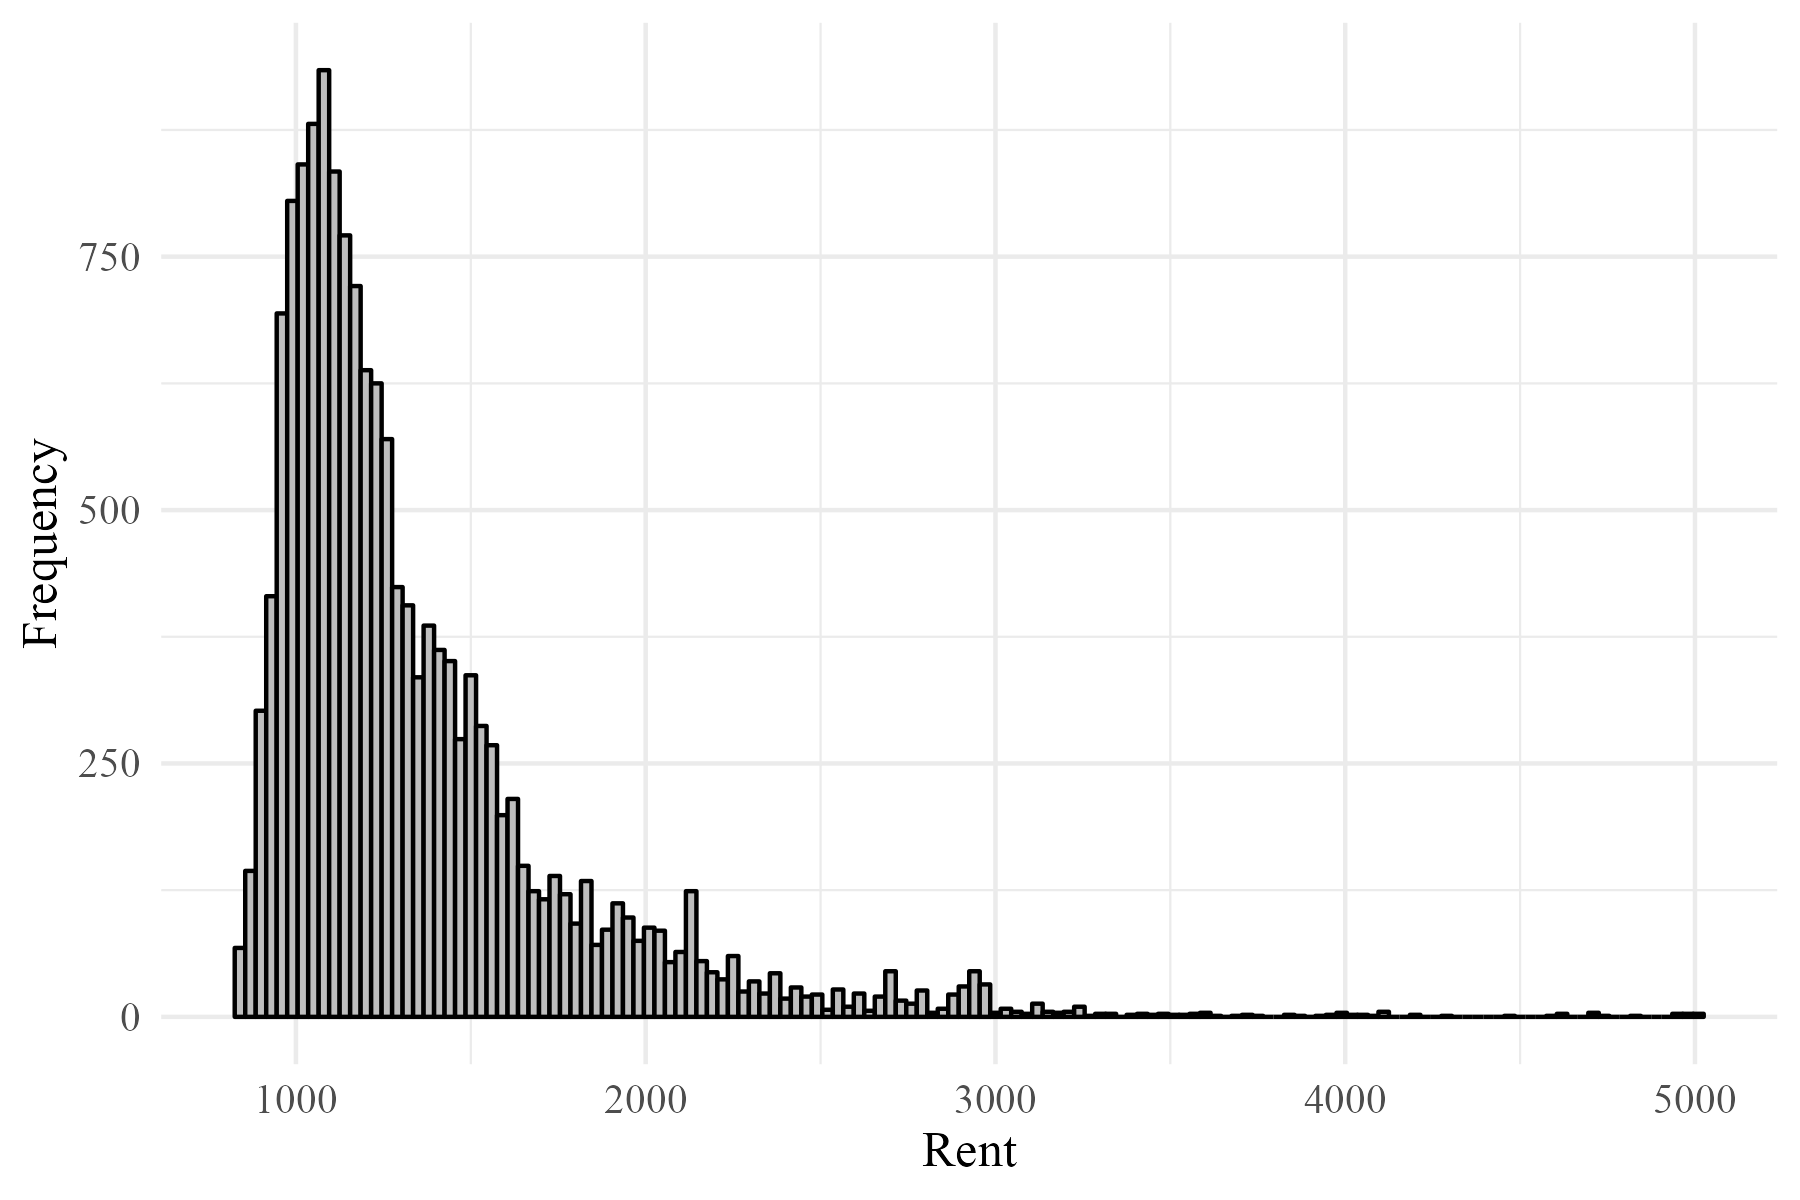
\includegraphics[width=1\linewidth]{hist.png}
\end{figure}
\clearpage


%----------------------------------------
% Figure 2
%----------------------------------------

\begin{figure}[p]
\caption{College Counties: \% Difference Between Median Rent and Avg Median Rent of State}
\label{fig:fig2}
\centering
\bigskip{}
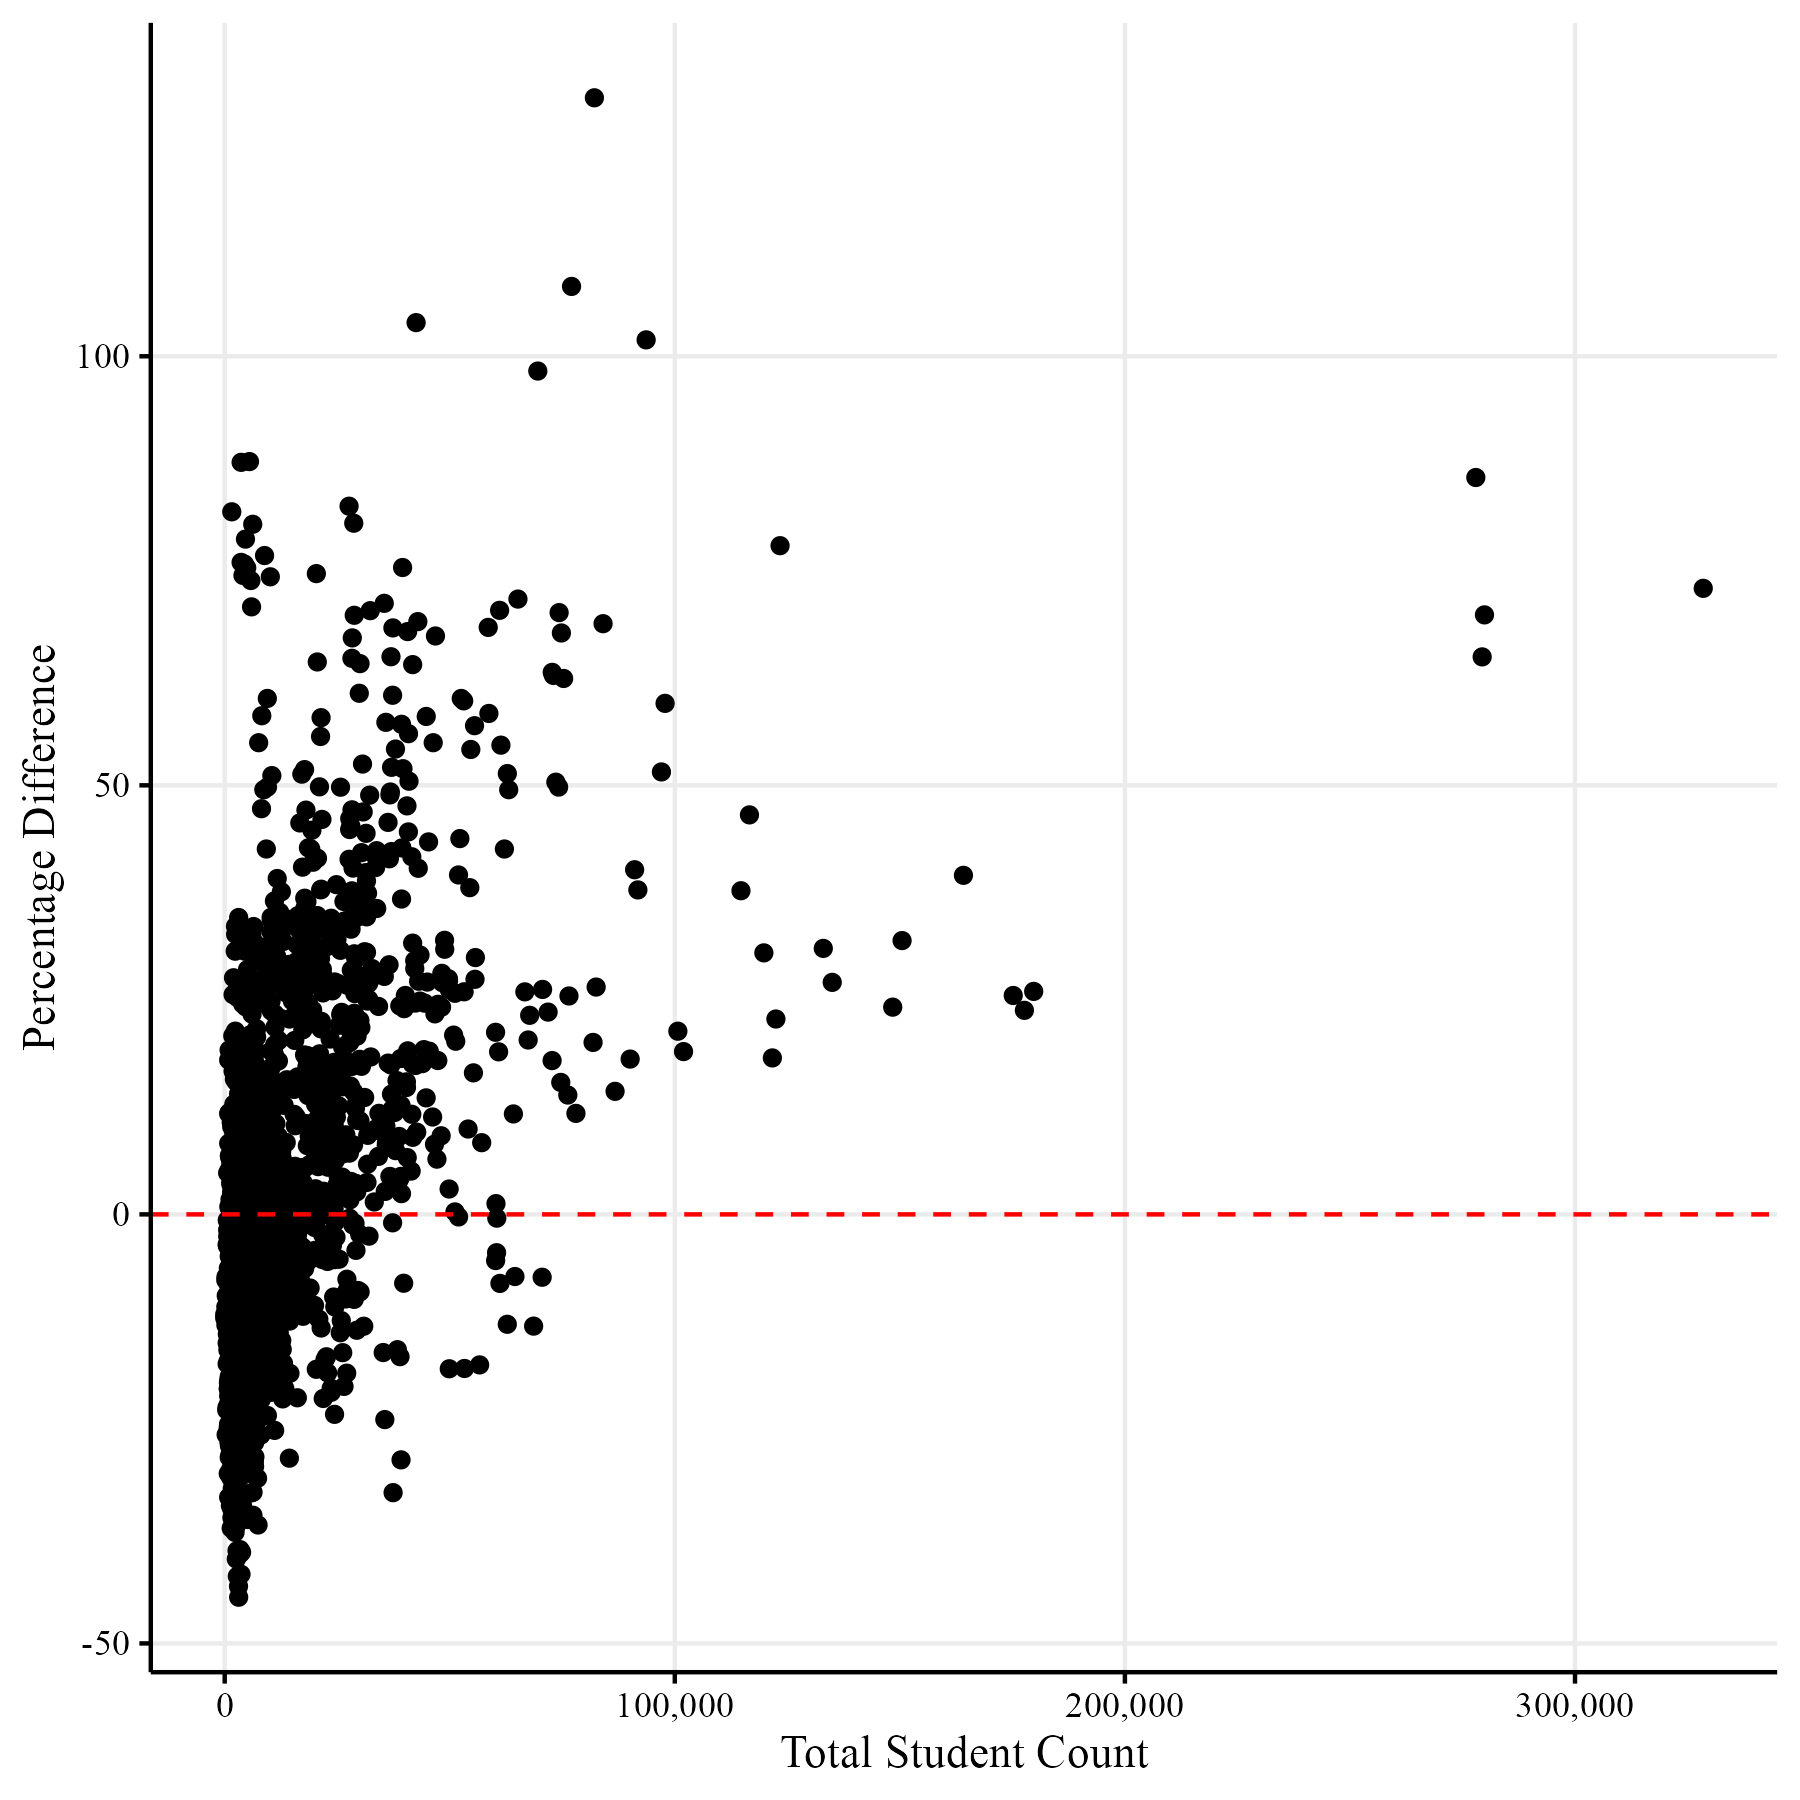
\includegraphics[width=1\linewidth]{totstud.png}
\end{figure}
\clearpage

%----------------------------------------
% Figure 3
%----------------------------------------

\begin{figure}[p]
\caption{College Counties: \% Difference Between Median Rent and Avg Median Rent of State}
\label{fig:fig3}
\centering
\bigskip{}
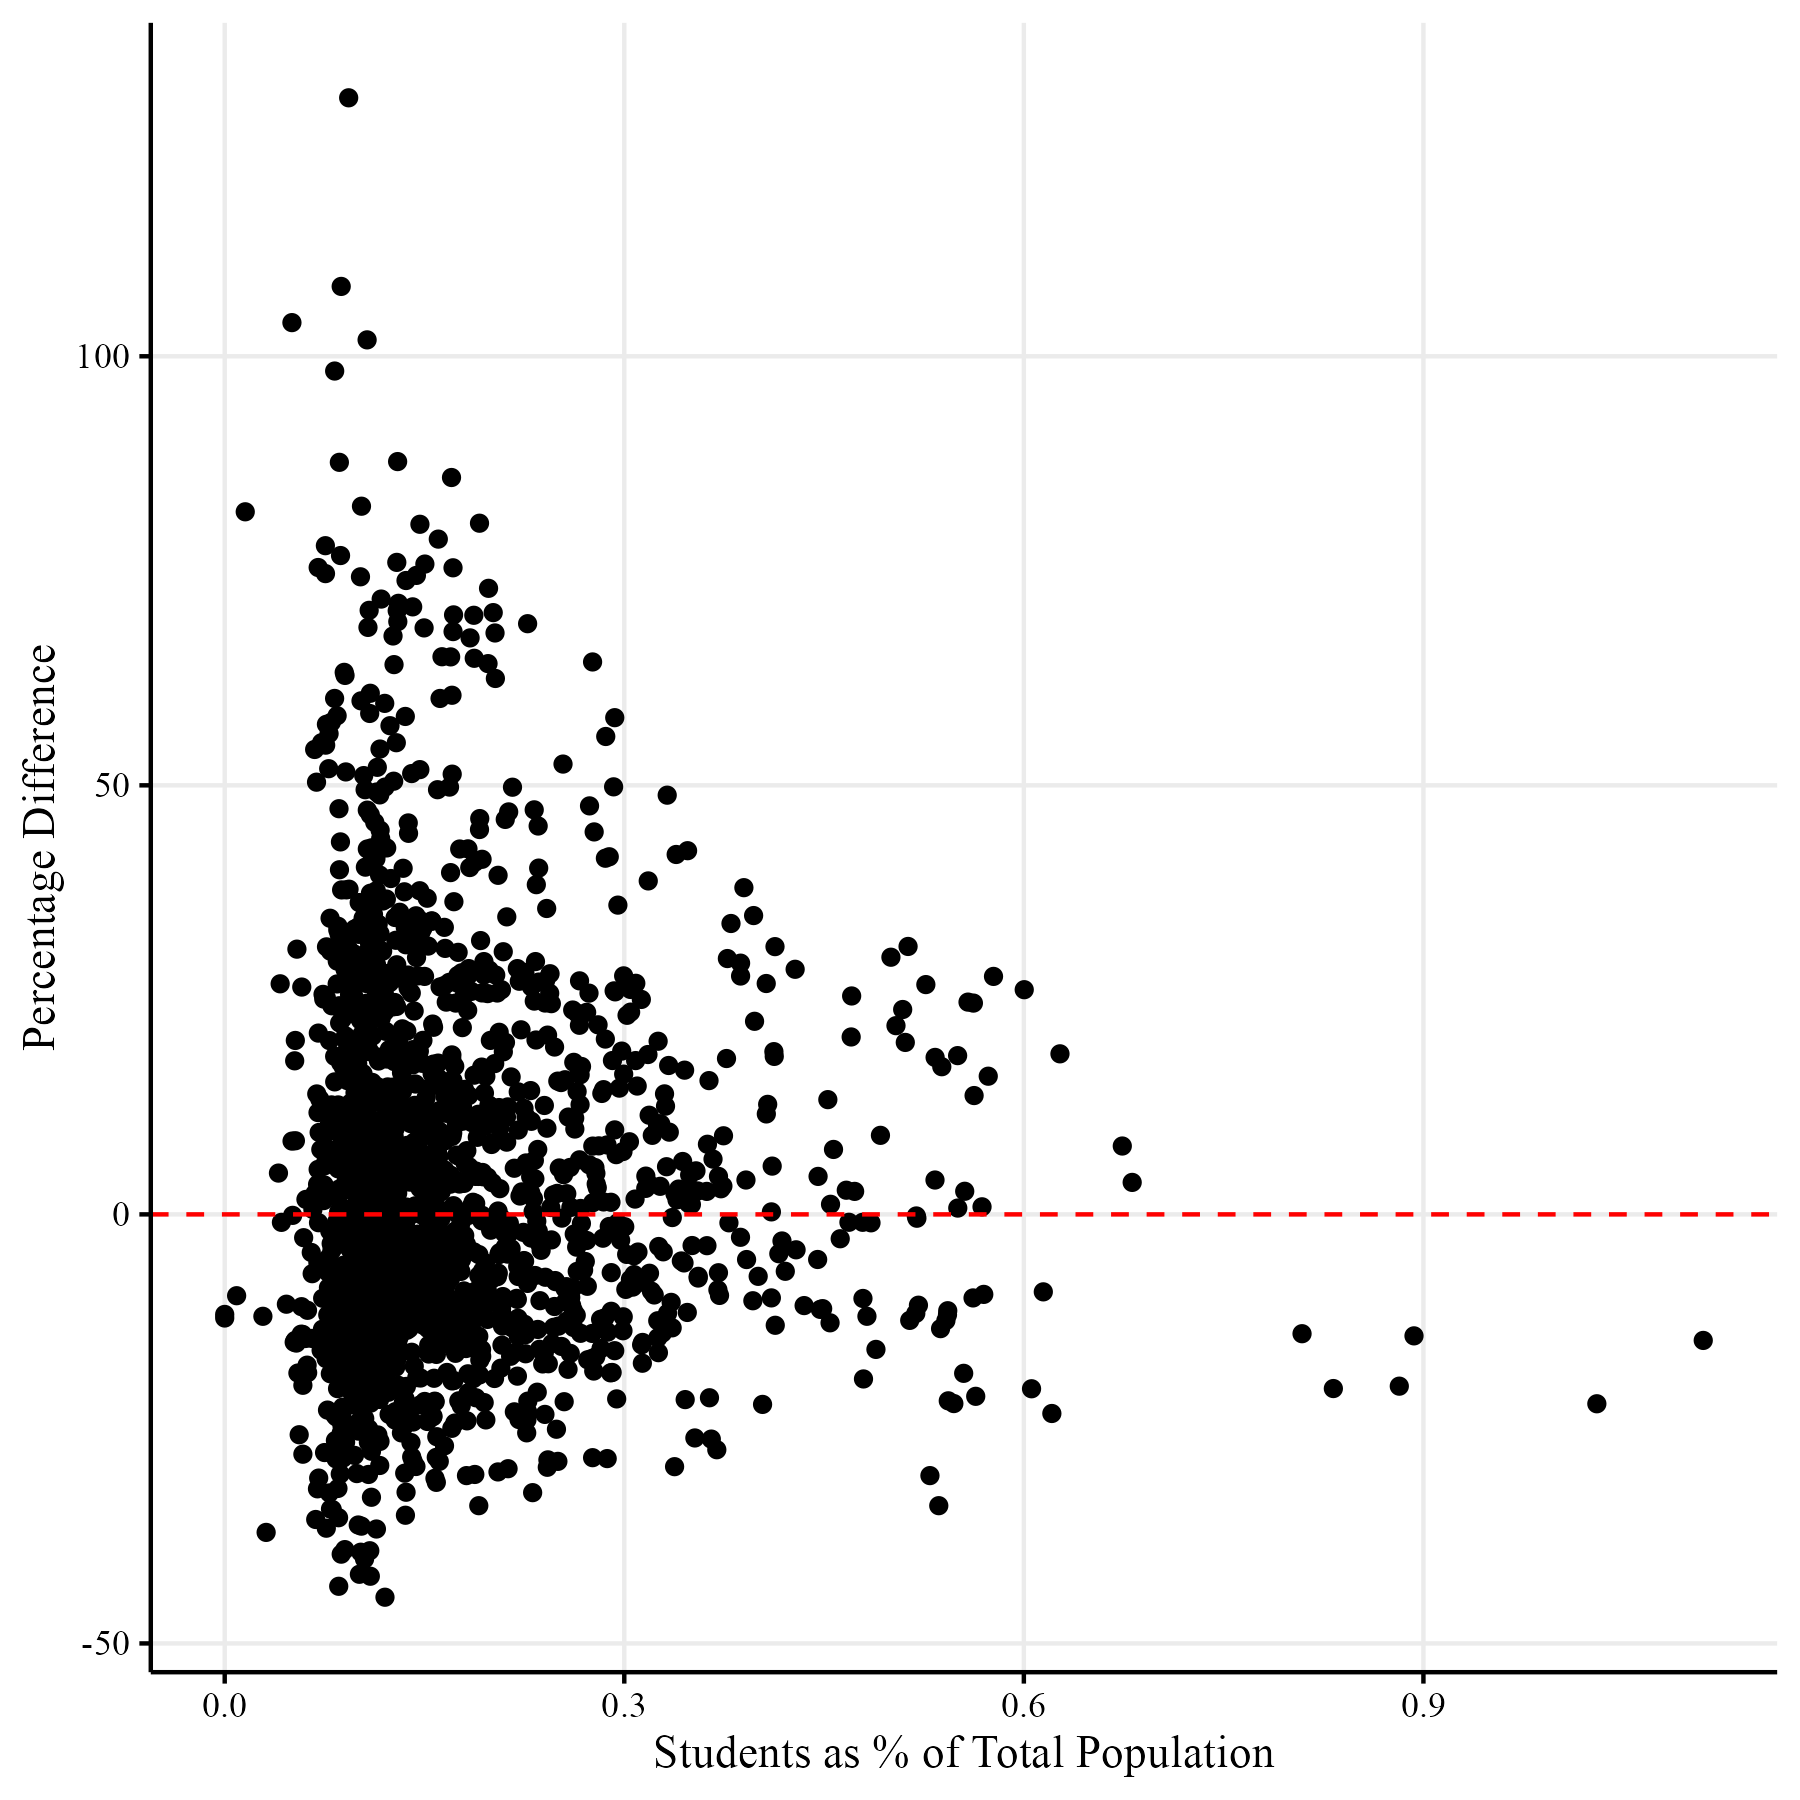
\includegraphics[width=1\linewidth]{pctstud.png}
\end{figure}
\clearpage

%----------------------------------------
% Table 3
%----------------------------------------

\begin{table*}[p]
\begin{adjustwidth}{-1in}{-1in} % adjust margins to center the table across the page
\caption{Pooled OLS Models}
\label{tab:olsmodels}
\centering
\begin{tabular}{lcccc}
\toprule
  & Model 1 & Model 2 & Model 3 (Any Stud.) & Model 4 (10\% Stud. Pop.)\\
\midrule
(Intercept) & \num{6.566}*** & \num{6.555}*** & \num{6.661}*** & \num{6.063}***\\
 & (\num{0.033}) & (\num{0.034}) & (\num{0.060}) & (\num{0.138})\\
Any Students & \num{-0.031}*** &  &  & \\
 & (\num{0.003}) &  &  & \\
10\% Student Population &  & \num{0.008}* &  & \\
 &  & (\num{0.004}) &  & \\
log(Total Students) &  &  & \num{-0.007}*** & \num{-0.022}\\
 &  &  & (\num{0.002}) & (\num{0.016})\\
Percent Students &  &  & \num{0.146}*** & \num{0.101}\\
 &  &  & (\num{0.030}) & (\num{0.069})\\
log(Total Population) & \num{-0.007} & \num{-0.011} & \num{-0.016} & \num{0.074}+\\
 & (\num{0.010}) & (\num{0.010}) & (\num{0.019}) & (\num{0.040})\\
log(Housing Units) & \num{0.052}*** & \num{0.051}*** & \num{0.078}*** & \num{0.002}\\
 & (\num{0.010}) & (\num{0.010}) & (\num{0.020}) & (\num{0.040})\\
Pop. Density & \num{0.000}*** & \num{0.000}*** & \num{0.000}*** & \num{0.000}+\\
 & (\num{0.000}) & (\num{0.000}) & (\num{0.000}) & \vphantom{2} (\num{0.000})\\
Median Income & \num{0.000}*** & \num{0.000}*** & \num{0.000}*** & \num{0.000}***\\
 & (\num{0.000}) & (\num{0.000}) & (\num{0.000}) & \vphantom{1} (\num{0.000})\\
Unemployment Rate & \num{0.001} & \num{0.001} & \num{-0.006}*** & \num{0.012}**\\
 & (\num{0.001}) & (\num{0.001}) & (\num{0.002}) & (\num{0.004})\\
Median Age & \num{-0.001}*** & \num{0.000} & \num{-0.004}*** & \num{-0.007}***\\
 & (\num{0.000}) & (\num{0.000}) & (\num{0.001}) & (\num{0.001})\\
Pct. Moved in Last Yr & \num{0.013}*** & \num{0.013}*** & \num{0.017}*** & \num{0.011}***\\
 & (\num{0.001}) & (\num{0.001}) & (\num{0.001}) & \vphantom{1} (\num{0.002})\\
Pct. Highly Educated & \num{0.004}*** & \num{0.003}*** & \num{0.002}*** & \num{0.006}***\\
 & (\num{0.000}) & (\num{0.000}) & (\num{0.000}) & \vphantom{3} (\num{0.001})\\
Pct. White & \num{-0.001}*** & \num{-0.001}** & \num{-0.001}* & \num{-0.001}\\
 & (\num{0.000}) & (\num{0.000}) & (\num{0.000}) & \vphantom{2} (\num{0.001})\\
Pct. Black & \num{0.001}*** & \num{0.001}*** & \num{0.002}*** & \num{0.001}\\
 & (\num{0.000}) & (\num{0.000}) & (\num{0.000}) & \vphantom{1} (\num{0.001})\\
Pct. Asian & \num{0.002}** & \num{0.002}*** & \num{-0.001} & \num{0.002}\\
 & (\num{0.001}) & (\num{0.001}) & (\num{0.001}) & (\num{0.002})\\
\midrule
Num.Obs. & \num{14731} & \num{14731} & \num{6957} & \num{1709}\\
R2 & \num{0.765} & \num{0.764} & \num{0.821} & \num{0.840}\\
R2 Adj. & \num{0.764} & \num{0.763} & \num{0.819} & \num{0.834}\\
AIC & \num{-17710.2} & \num{-17615.4} & \num{-8964.8} & \num{-2632.1}\\
BIC & \num{-17185.9} & \num{-17091.1} & \num{-8485.5} & \num{-2272.8}\\
Log.Lik. & \num{8924.075} & \num{8876.690} & \num{4552.391} & \num{1382.035}\\
F &  &  & \num{463.588} & \num{134.912}\\
RMSE & \num{0.13} & \num{0.13} & \num{0.13} & \num{0.11}\\
\bottomrule
\multicolumn{5}{l}{\rule{0pt}{1em}+ p $<$ 0.1, * p $<$ 0.05, ** p $<$ 0.01, *** p $<$ 0.001}\\
\end{tabular}
\end{adjustwidth}
\end{table*}
\clearpage
%----------------------------------------
% Table 4
%----------------------------------------
\begin{table*}[p]
\begin{adjustwidth}{-1in}{-1in} % adjust margins to center the table across the page
\caption{Fixed Effects Models}
\label{tab:femodels}
\centering
\begin{tabular}[t]{lccc}
\toprule
  & Model 5 (All Counties) & Model 6 (Any Students) & Model 7 (10\% Student Counties)\\
\midrule
Total Students & \num{0.000}+ &  & \\
 & (\num{0.000}) &  & \\
Percent Students & \num{0.008} & \num{0.007} & \num{0.031}\\
 & (\num{0.030}) & (\num{0.030}) & (\num{0.048})\\
log(Total Students) &  & \num{0.001} & \num{-0.005}\\
 &  & (\num{0.003}) & (\num{0.011})\\
log(Population) & \num{0.097}*** & \num{0.098}* & \num{0.019}\\
 & (\num{0.024}) & (\num{0.045}) & (\num{0.081})\\
log(Housing Units) & \num{0.144}*** & \num{0.187}*** & \num{0.219}***\\
 & (\num{0.018}) & (\num{0.034}) & (\num{0.066})\\
Pop. Density & \num{0.000}** & \num{0.000}** & \num{0.000}\\
 & (\num{0.000}) & (\num{0.000}) & \vphantom{2} (\num{0.000})\\
Median Income & \num{0.000}*** & \num{0.000}*** & \num{0.000}***\\
 & (\num{0.000}) & (\num{0.000}) & \vphantom{1} (\num{0.000})\\
Unemployment Rate & \num{0.006}*** & \num{0.003}* & \num{0.009}**\\
 & (\num{0.001}) & (\num{0.001}) & (\num{0.003})\\
Median Age & \num{-0.002}* & \num{0.003} & \num{0.001}\\
 & (\num{0.001}) & (\num{0.002}) & \vphantom{1} (\num{0.004})\\
Pct. Moved in Last Yr & \num{-0.001} & \num{-0.007}*** & \num{-0.011}**\\
 & (\num{0.001}) & (\num{0.002}) & (\num{0.004})\\
Pct. Highly Educated & \num{0.000} & \num{-0.002} & \num{-0.010}***\\
 & (\num{0.001}) & (\num{0.001}) & (\num{0.002})\\
Pct. White & \num{-0.004}*** & \num{0.000} & \num{0.008}\\
 & (\num{0.001}) & (\num{0.002}) & \vphantom{2} (\num{0.005})\\
Pct. Black & \num{0.002}+ & \num{0.001} & \num{0.009}+\\
 & (\num{0.001}) & (\num{0.002}) & \vphantom{1} (\num{0.005})\\
Pct. Hispanic & \num{-0.003}* & \num{0.014}*** & \num{0.012}\\
 & (\num{0.001}) & (\num{0.003}) & (\num{0.008})\\
\midrule
Num.Obs. & \num{14739} & \num{6962} & \num{1709}\\
R2 & \num{0.335} & \num{0.441} & \num{0.333}\\
R2 Adj. & \num{0.164} & \num{0.298} & \num{0.154}\\
AIC & \num{-50629.6} & \num{-25028.5} & \num{-5951.0}\\
BIC & \num{-50477.6} & \num{-24891.6} & \num{-5842.1}\\
RMSE & \num{0.04} & \num{0.04} & \num{0.04}\\
\bottomrule
\multicolumn{4}{l}{\rule{0pt}{1em}+ p $<$ 0.1, * p $<$ 0.05, ** p $<$ 0.01, *** p $<$ 0.001}\\
\end{tabular}
\end{adjustwidth}
\end{table*}

\end{document}